\chapter{Sets and Logic}

The use of math usually falls into two categories:
\begin{itemize}
\item \textit{Developing mathematical tools that let us make better predictions.}  This is how engineers and scientists use math.  It is usually referred to as \newterm{applied math}.
\item \textit{Creating interesting statements and proving them to be true or false.}  This is known as \newterm{pure math}.
\end{itemize}

Many mathematical ideas start out as pure math, and eventually
become useful. For example, the field of number theory is devoted to
proving things about prime numbers.  The mathematicians who created
number theory were certain that it could never be used for any
practical purpose.  After a century or two, number theory was used as
the basis of most cryptography systems.

Conversely, some ideas start out as a "rule of thumb" that engineers use, and are
eventually rigorously defined and proven.

This course tends to emphasize applied math, but you should know
something about the tools of pure math.

You can think of all the mathematical proofs as a tree. Each proof
proves some statement true. To do this, the proof uses logic and
statements that were proven true by other truths. So, the tree is built
from the bottom up.  However, the tree has to have a bottom. At the
very bottom of the tree are some statements that we just accept as
true without proof.  These are known as \newterm{axioms}.

All of modern mathematics can be built from:
\begin{itemize}
\item A short list of axioms.
\item A few rules of logic.
\end{itemize}

There have been several efforts to codify a small but complete
axiomatic system. The most popular one is known as \newterm{ZFC}.  "Z"
is for the Ernst Zermelo, who did most of the work.  "F" is for
Abraham Fraenkel, who tidied up a couple of things. "C" is for The
Axiom of Choice.  As a community, mathematicians debate whether the
Axiom of Choice should be an axiom; we get a couple of strange results
if we include it in the system.  If we do not, there are a few obviously
useful ideas that we can't prove true.

ZFC has 10 axioms.  We simply accept these 10 statements as true, and
all the proofs of modern mathematics can be extrapolated from them.
The 10 axioms are all stated in terms of sets.

\section{Sets}

A \newterm{set} is a collection.  For example, you might talk about the set of
odd numbers greater than 5, or the set of all protons in the
universe.  \index{set}

We have a notation for sets.  For example, here is how we define $S$ to
be the set containing 1, 2, and 3:

$$S = \{1, 2, 3\}$$

We say that 1, 2, and 3 are \newterm{elements} of the set $S$.
(Sometimes we will also use the word "member")

If you want to say "2 is an element of the set $S$" in mathematical
notation, it is done like this:

$$ 2 \in S$$

If you want to say "5 is \textit{not} an element of the set $S$", it
looks like this:

$$ 5 \notin S$$

We have notation for a few sets that we use all the time:

\begin{tabular}{c|c}
Set & Symbol \\
\hline
The empty set & $\emptyset$ \\ \index{$\emptyset$}
Natural numbers & $\mathbb{N}$ \\ \index{$\mathbb{N}$}
Integers & $\mathbb{Z}$ \\ \index{$\mathbb{Z}$}
Rational numbers & $\mathbb{Q}$ \\ \index{$\mathbb{Q}$}
Real numbers & $\mathbb{R}$ \\ \index{$\mathbb{R}$}
Complex numbers & $\mathbb{C}$ \index{$\mathbb{C}$}
\end{tabular}

The empty set is the set that contains nothing.  It is also sometimes
called \newterm{the null set}.

Often, when we define a set, we start with one of these big sets and
say "The set I'm talking about is the members of the big set, but only
the one for which this statement is true".  For example, if you wanted
to talk about all the integers greater than or equal to -5, you could
do it like this:

$$A = \{ x \in \mathbb{Z} \mid x \geq -5 \}$$

When you read this aloud, you say "$A$ is the set of integers $x$
where $x$ is greater than or equal to negative 5."

\subsection{And and Or}

Sometimes you need the members to satisfy two conditions; for this, we
use "and": \index{and}

$$A = \{ x \in \mathbb{Z} \mid x > -5 \text{ and }  x < 100\}$$

This is the set of integers that are greater than -5 \textit{and} less
than 100.  In this book, we usually just write "and", but if you do a
large amount of set and logic work, you will use the symbol $\land$:

$$A = \{ x \in \mathbb{Z} \mid (x > -5) \land (x < 100)\}$$

Sometimes, you want a set that satisfies at least one of two
conditions.  For this, you use "or":\index{or}

$$A = \{ x \in \mathbb{Z} \mid x < -5 \text{ or } x > 100\}$$

These are the number that are less than -5 or greater than 100.  Once
again, there is a symbol for this:

$$A = \{ x \in \mathbb{Z} \mid (x < -5) \lor (x > 100)\}$$

\subsection{How simple are sets?}

Sets are so simple that some questions just don't make any sense:
\begin{itemize}
\item "What is the first item in the set?" makes no sense to a mathematician.  Sets have no order.
\item "How many times does the number 6 appear in the set?"  makes no sense.   6 is a member, or it is not.   
\end{itemize}

\subsection{Subsets}

If every member of set $A$ is also in set $B$, we say that "$A$ is a
subset of $B$." \index{subset}

For example, if $A = \{1,4,5\}$ and $B = \{1,2,3,4,5,6\}$, then $A$ is
a subset of $B$.  There is a symbol for this:

$$ A \subseteq B$$

Remember the table of commonly used sets?  We can arrange them as
subsets of each other:

$$\emptyset \subseteq \mathbb{N} \subseteq \mathbb{Z} \subseteq \mathbb{Q} \subseteq \mathbb{R} \subseteq \mathbb{C}$$

Note that that subsets have the transitive property: $\mathbb{N}
\subseteq \mathbb{Z} \subseteq \mathbb{Q}$ thus $\mathbb{N} \subseteq
\mathbb{Q}$

Note that if $A$ and $B$ have the same elements, $A \subseteq B$
\textit{ and } $B \subseteq A$. In this case, we say that the two sets
are equal.

We also have a symbol for "is not a subset of": $A \not\subset B$

\subsection{Union and Intersection of Sets}

If you have two sets $A$ and $B$, you might want to say "Let $C$ be
the set containing element that are in \textit{either} $A$ or $B$."
We say that $C$ is the \newterm{union} of $A$ and $B$.  There is
notation for this too:\index{union}

$$C = A \cup B$$

For example,  if $A = \{1,3,4,9\}$ and $B = \{3,4,5,6,7,8\}$,  then $A \cup B =  \{1,3,4,5,6,7,8,9\}$.

You also want to say "Let $C$ be the set containing elements that are
in \textit{both} $A$ and $B$."  We say that $C$ is the
\newterm{intersection} of $A$ and $B$.  There is notation for this
too:\index{intersection}

$$C = A \cap B$$

For example,  if $A = \{1,3,4,9\}$ and $B = \{3,4,5,6,7,8\}$,  then $A \cap B =  \{3,4\}$.

\subsection{Venn Diagrams}

When discussing sets, it is often helpful to have a Venn diagram to
look at.  Venn diagrams represent sets as circles. For example, the
sets $A$ and $B$ above could look like this:\index{Venn diagrams}

\begin{tikzpicture}[fill=gray]
\draw (0,0) circle (3) (0,3)  node [text=black,above] {$A$};
\draw (3,0) circle (3) (3,3)  node [text=black,above] {$B$};
\draw (-1.5,0) node [above] {$1, 9$};
\draw (1.5, 0) node [above] {$3,4$};
\draw (4.5, 0) node [above] {$5,6,7,8$};
\end{tikzpicture}

It makes it easy to see that $A$ and $B$ have a non-empty
intersection, but they are not subsets of each other.

Often we won't even show the individual elements. For example, in the
universe of all polygons, some rectangles are squares. Here's the Venn diagram:

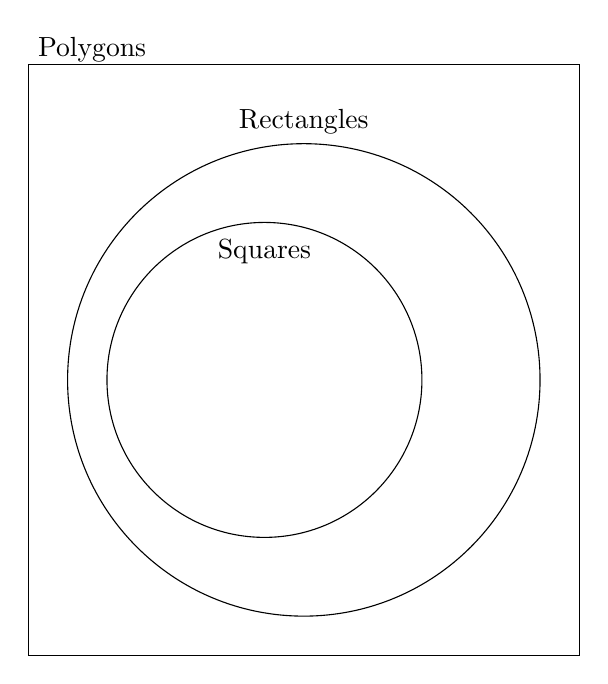
\begin{tikzpicture}[fill=gray]
  \draw (-3.5,-3.5) rectangle (3.5,4.0);
  \draw (-3.5, 4.2) node [above,right] {Polygons};
  \draw (0,0) circle (3) (0,3)  node [above] {Rectangles};
  \draw (-0.5,0) circle (2) (-0.5,1.9)  node [below] {Squares};
\end{tikzpicture}

As the combinations get more complex, we sometimes use shading to
indicate what part we are talking about.  For example, imagine we
wanted all the rectangles with area greater than 5.0 that are not
squares.  The diagram might look like this:

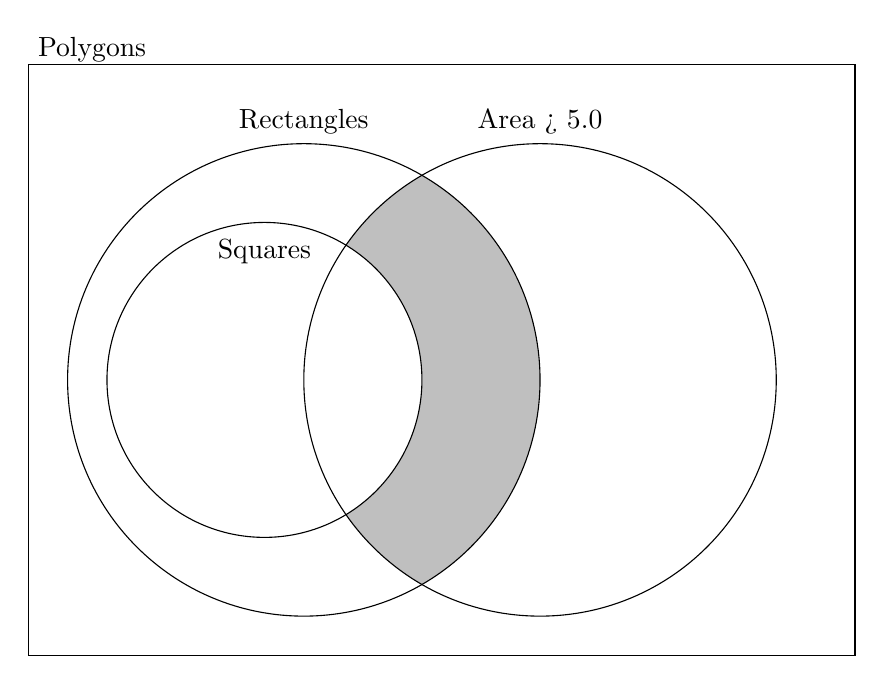
\begin{tikzpicture}[fill=lightgray]
  \draw (-3.5,-3.5) rectangle (7,4.0);
  \scope
  \clip (0,0) circle (3);
  \fill (3,0) circle (3);
  \fill [white] (-0.5,0) circle (2);
  \endscope
  \draw (-3.5, 4.2) node [above,right] {Polygons};
  \draw (0,0) circle (3) (0,3)  node [above] {Rectangles};
  \draw (-0.5,0) circle (2) (-0.5,1.9)  node [below] {Squares};
  \draw (3,0) circle (3) (3,3)  node [above] {Area > 5.0};
\end{tikzpicture}


\section{Logic}

We use a lot of logic in set theory.  For example, the shaded region
above represents all the polygons for which all the following are
true:\index{logic}
\begin{itemize}
\item It is a rectangle.
\item It is \textit{not} a square.
\item It has an area greater than 5.0.
\end{itemize}

\section{Implies}

In logic, we will often say ``$a$ implies $b$''.  That means ``If the
statement $a$ is true, the statement $b$ is also true.''  For example:
``$p$ is a square'' implies ``$p$ is a rectangle''.\index{implies}

There is notation for this: an arrow in the direction of the implication.

$$p \text{ is a square } \implies p \text{ is a rectangle}$$

Notice that implication has a direction: ``$p$ is a rectangle'' does \textit{not} imply 
``$p$ is a square''.

Implications can be chained together: If $A \implies B$ and $B \implies C$,  then $A \implies C$.

\section {If and Only If}

If the implication goes both ways, we use ``if and only if''.  This
means the two conditions are equivalent.  For example: ``$n$ is even
if and only if there exists an integer $m$ such that $2m = n$''. \index{if and only if}

There is a notation for this too:

$$p \text{ is even } \iff \text{ there exists an integer } m \text{ such that } 2m = n$$

There is even notation for ``there exists''. It is a backwards capital E:

$$p \text{ is even } \iff \exists m \in \mathbb{Z}  \text{ such that } 2m = n$$

\section {Not}

The not operation flips the truth of an expression:\index{not}
\begin{itemize}
\item If $a$ is true, $\text{not}(a)$ is false.

\item If $a$ is false, $\text{not}(a)$ is true.
\end{itemize}

We sometimes talk about ``notting'' or ``negating'' a value.  We won't
use it much, but there is a symbol for this: $\neg$.

We might create a \newterm{logic table} for negation that shows all
the possible values and their negation:

\begin{tabular}{c | c}
  $A$ & $\neg A$ \\
  \hline
  F & T \\
  T & F
\end{tabular}

This table says ``If $A$ is false, $\neg A$ is true. If $A$ is true,
$\neg A$ is false.''

Most logic tables are for operations that take more than one input.
For example, this logic table shows the values for and-ing and or-ing:

\begin{tabular}{c | c | c | c}
  $A$ & $B$ & $A \text{ and } B$ & $A \text{ or } B$ \\
  \hline
  F & F & F & F \\
  F & T & F & T \\
  T & F & F & T \\
  T & T & T & T \\
\end{tabular}

Notice that we have to enumerate all possible combinations of the
inputs of $A$ and $B$.

When a variable like $A$ can only take two possible values, we say it
is a \newterm{boolean} variable. (George Bool did important work in
this area.)

\begin{Exercise}[title={Logic Table}, label=logic_table]

  Make a logic table that enumerates all possible combinations of boolean variables $A$ and $B$ and shows the value of the two following expressions:
  \begin{itemize}
  \item $\neg \left(A \text{ or } B \right)$
  \item $\left(\neg A \right) \text{ and } \left(\neg B \right)$ 
  \end{itemize}

\end{Exercise}

\begin{Answer}[ref=logic_table]

\begin{tabular}{c | c | c | c}
  $A$ & $B$ & $\text{ not} \left(A \text{ or } B \right)$
  & $\left(\text{ not } A \right) \text{ and } \left(\text{ not } B \right)$ \\
  \hline
  F & F & T & T \\
  F & T & F & F \\
  T & F & F & F \\
  T & T & F & F \\
\end{tabular}

Notice that the two expressions are equivalent!

DeMorgan's Rule says ``$\text{not } \left(A \text{ or } B \right)$'' is
equivalent to ``$\left(\text{not } A \right) \text{ and } \left(\text{not } B
\right)$''.

It also says ``$\text{not } \left(A \text{ and } B \right)$'' is
equivalent to ``$\left(\text{not } A \right) \text{ or } \left(\text{not } B\right)$''.

\end{Answer}

\section{Cardinality}

Informally, the \newterm{cardinality} of a set is the number of
elements it contains. So, $\{1,3,5\}$ has a cardinality of 3.  The
null set has a cardinality of zero.\index{cardinality}

Things get a little trickier if a set is infinite.  We say two
infinite sets $A$ and $B$ have the same cardinality if there is some
mapping that pairs every member of $A$ with a member of $B$ and
mapping that pairs every member of $B$ with a member of $A$.

\section{Complement of a Set}

Most sets exist in a particular universe, for example you might talk
about the even numbers as a set in the integers. You can then talk
about the set's \newterm{complement}: the set of everthing else. For
example, the complement of the even numbers (inside the integers) is
the odd numbers.

If you have a set $A$, its complement is usually denoted by $A'$.

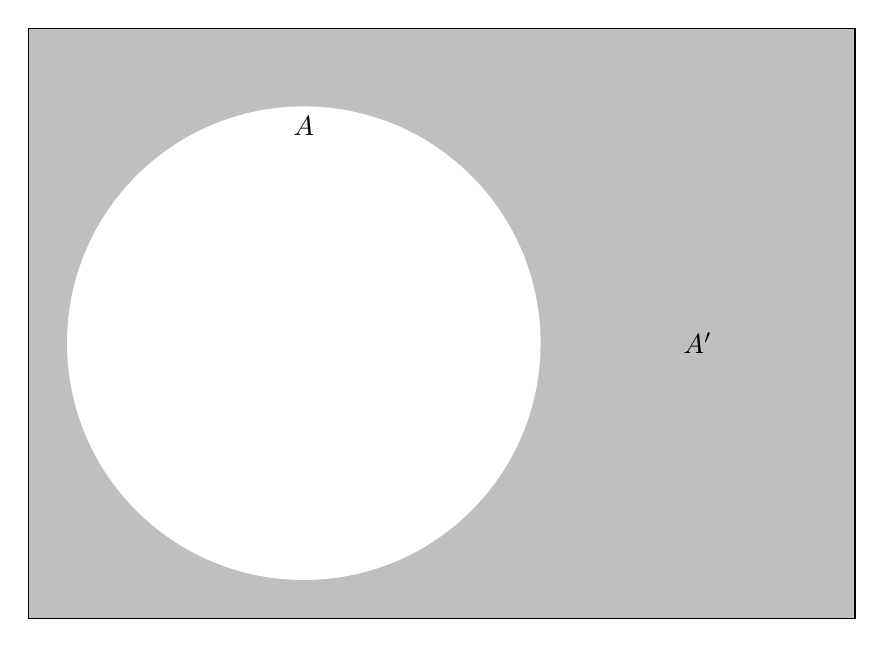
\begin{tikzpicture}[fill=lightgray]
\filldraw (-3.5,-3.5) rectangle (7,4.0);
\filldraw [white] (0,0) circle (3) (0,3)  node [text=black,below] {$A$};
\draw (5,0) node {$A'$};
\end{tikzpicture}

\section{Subtracting Sets}

If you have sets $A = \{1,2,3,4\}$ and $B = \{1, 4\}$, it makes sense
to subtract $B$ from $A$ by removing 1 and 4 from $A$.

If $A$ and $B$ are sets, we define $A - B$ to be $A \cap B'$.  Take a
second to look at this diagram and convince yourself that the white
region represents $A - B$ and that it is the same as $A \cap B'$.

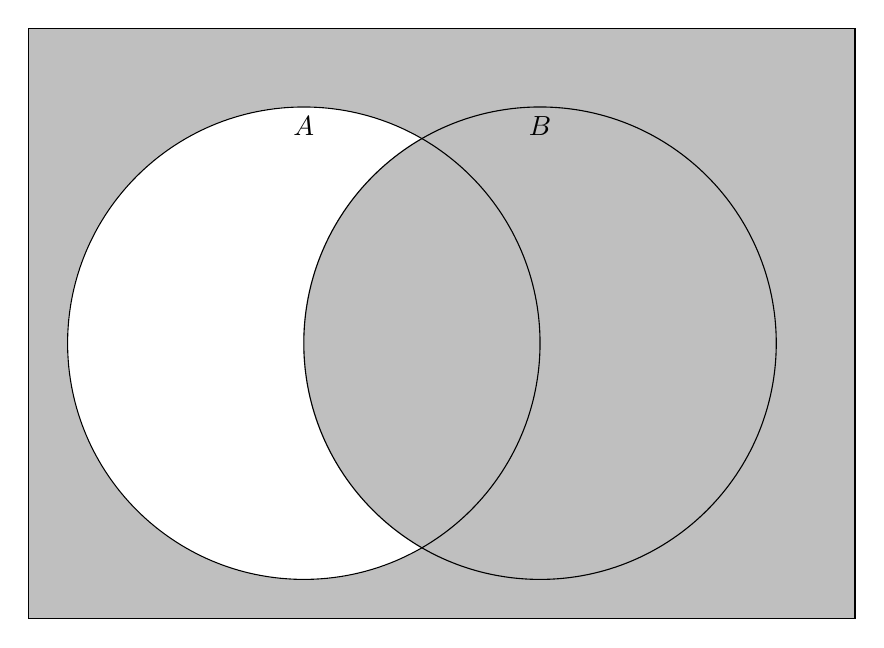
\begin{tikzpicture}[fill=lightgray]
\filldraw (-3.5,-3.5) rectangle (7,4.0);
\filldraw [white] (0,0) circle (3);
\filldraw [lightgray] (3,0) circle (3);
\draw [black] (0,0) circle (3) (0,3)  node [text=black,below] {$A$};
\draw [black] (3,0) circle (3) (3,3)  node [text=black,below] {$B$};
\end{tikzpicture}

\section{Power Sets}

It is not uncommon to have a set whose elements are also sets.  For
example, you might have the set that contains the following two sets:
$\{1,2,3\}$ and $\{2,3,4\}$. You might write it like this: $\{
\{1,2,3\}, \{2,3,4\} \}$. (Note that this set has a cardinality of 2
--- it has two members that are sets.)\index{sets of sets}

Given any set $A$, you can construct its \newterm{power set}, which is
the set of all subsets of $A$.  For example, if you have a set
$\{1,2,3\}$, its power set is $\{\{1,2,3\}, \{1,2\},\{1,3\}, \{2,3\},
\{1\}, \{2\}, \{3\}, \emptyset\}$.\index{power set}

If a set has $n$ elements, its power set has $2^n$ elements.

\section{Booleans in Python}

In Python, we can have variables hold boolean values: \texttt{True}
and \texttt{False}.  We also have operators: \texttt{not},
\texttt{and}, and \texttt{or}.\index{boolean variables}

For example, you could find out what the expression ``$a$ and not
$b$'' is if both variables are false like this:
\begin{verbatim}
a = False
b = False
result = a or not b
print(f"a={a}, b={b}, a or not b = {result}")
\end{verbatim}

This would print out:
\begin{verbatim}
a=False, b=False, a or not b = True
\end{verbatim}

What if you wanted to try all possible values for \texttt{a} and
\texttt{b}? You could use \texttt{itertools}.

\begin{verbatim}
import itertools

all_combos = itertools.product([False, True], repeat=2)
for (a, b) in all_combos:
    result = a or not b
    print(f"a={a}, b={b}: a or not b = {result}")       
\end{verbatim}

Type it in and run it. You should get the whole logic table:

\begin{verbatim}
a=False, b=False: a or not b = True
a=False, b=True: a or not b = False
a=True, b=False: a or not b = True
a=True, b=True: a or not b = True
\end{verbatim}

If you had three inputs into the expression, your truth table would
have eight entries.  For example, if you wanted to know the truth
table for $a and not(b and c)$, here is the code:

\begin{verbatim}
all_combos = itertools.product([False, True], repeat=3)
for (a, b, c) in all_combos:
    result = a and not(b and c)
    print(f"a={a}, b={b}, c={c}: a and not (b and c) = {result}")
\end{verbatim}

Type it in and run it. You should get:

\begin{verbatim}
a=False, b=False, c=False: a and not (b and c) = False
a=False, b=False, c=True: a and not (b and c) = False
a=False, b=True, c=False: a and not (b and c) = False
a=False, b=True, c=True: a and not (b and c) = False
a=True, b=False, c=False: a and not (b and c) = True
a=True, b=False, c=True: a and not (b and c) = True
a=True, b=True, c=False: a and not (b and c) = True
a=True, b=True, c=True: a and not (b and c) = False
\end{verbatim}

\section{The Contrapositive}

Here is a statement with an implication: ``If it has rained in the last hour, the grass is wet.''

This is \textit{not} equivalent to ``If the grass is wet, it has
rained in the last hour.'' (After all, the sprinkler may be running.)

However, it is exactly equivalent to its \newterm{contrapositive}:
``If the grass is not wet, it has not rained in the last hour.'' \index{contrapositive}

The rule can be written using symbols:

$$\left( A \implies B \right) \iff \left( \neg B \implies \neg A \right)$$

\section{The Distributive Property of Logic}

Many ideas from integer arithmetic have analogues in boolean
arithmetic. For example, there is a distributive property for booleans.  These two expressions are equivalent:
\begin{itemize}
  \item $A \text{ and } \left(B \text{ or } C \right)$
  \item $\left(A \text{ and } B \right) \text{ or } \left( A \text{ and } C \right)$
\end{itemize}

So are these:

\begin{itemize}
  \item $A \text{ or } \left(B \text{ and } C \right)$
  \item $\left(A \text{ or } B \right) \text{ and } \left( A \text{ or } C \right)$
\end{itemize}


\section{Exclusive Or}

The expression ``$a \text{ or } b$'' is true in any of the following conditions:
\begin{itemize}
\item $a$ is True and $b$ is False.
\item $a$ is False and $b$ is True.
\item Both $a$ and $b$ are True.
\end{itemize}

Sometimes engineers need a way to say ``Either $a$ or $b$ is true, but not
both.'' For this, we use \newterm{exclusive OR} (or XOR).\index{XOR}

Here, then, is the logic table for XOR

\begin{tabular}{c | c | c}
  $A$ & $B$ & XOR($a$,$b$) \\
  \hline
  F & F & F \\
  F & T & T \\
  T & F & T \\
  T & T & F \\
\end{tabular}

In Python, Logical XOR is done using \texttt{!=}:

\begin{verbatim}
just_one = (a != b)
\end{verbatim}

(Take 10 seconds to confirm that this is the same as the logic table
above.)


